\chapter{Usage au quotidien}
\label{ch:usage}

Ce chapitre parcourt les flux que vous lancerez des dizaines de
fois une fois la bibliothèque opérationnelle : cataloguer un nouveau
volume, chercher dans la collection, déplacer un volume, le prêter,
le récupérer, et auditer ce qui est sur les étagères.

\section{La barre latérale}\label{sec:navbar}

Dans une fenêtre d'au moins 1024\,px de large, la navigation occupe
une \emph{barre latérale}\index{barre latérale} à gauche de la page ;
elle reste en place quand la page défile. Ses entrées sont réunies en
groupes séparés par un filet : \textbf{Accueil} ; puis
\textbf{Catalogue}, \textbf{Emplacements} et \textbf{Séries} ; puis,
pour les Bibliothécaires et les Admins, \textbf{Emprunteurs},
\textbf{Prêts}, \textbf{Wish list}, \textbf{Étiquettes} et
\textbf{Propositions} ; enfin, pour les seuls Admins, \textbf{Admin}.
La page où vous vous trouvez est en gras, marquée d'un trait de
couleur sur sa gauche. L'entrée \textbf{Propositions} porte un badge
qui compte les propositions en attente de décision (\texttt{99+}
au-delà de 99 ; chapitre~\ref{ch:agents}).

Le pied de la barre réunit le choix de la langue, le bouton de thème
et \textbf{Déconnexion} (ou \textbf{Connexion} pour un visiteur
anonyme). En dessous, le bouton \textbf{Réduire le menu} ramène la
barre à une colonne d'icônes, ce qui laisse plus de place à la page ;
le nom de chaque entrée apparaît alors dans une infobulle quand la
souris survole l'icône ou que la touche Tab l'atteint, et le badge des
propositions devient une pastille posée sur l'icône. Le même bouton
redéploie la barre. Le navigateur retient ce choix : la page suivante,
comme la visite suivante, s'ouvre dans le même état. Le choix est
propre au navigateur et non au compte --- un autre ordinateur garde le
sien.

\paragraph{Sur un téléphone ou dans une fenêtre étroite.} En dessous
de 1024\,px, la barre latérale disparaît ; une fine barre reste en
haut de la page, avec le bouton de \textbf{menu} (trois traits
horizontaux) et le logo mybibli. Le bouton de menu ouvre la même
navigation dans un tiroir qui glisse depuis la gauche par-dessus la
page assombrie : mêmes entrées, même badge, et au pied le choix de la
langue, le bouton de thème et Déconnexion (ou Connexion) ; le tiroir
n'est jamais réduit. On le referme avec Échap, d'un appui sur la page
assombrie, avec le bouton de fermeture en haut du tiroir, ou en
suivant l'un de ses liens. Tant qu'il est ouvert, la page derrière lui
ne défile pas et ne reçoit pas le clavier, et une lecture de la
douchette est ignorée au lieu d'aboutir dans le champ de scan.

\paragraph{Thème clair ou sombre.} Le bouton de thème fait passer
toute l'interface du clair au sombre et inversement. Le navigateur
retient ce choix ; tant que vous n'en avez fait aucun, mybibli suit
le réglage du système de l'appareil. L'impression est toujours
claire, quel que soit le thème à l'écran.

\section{La page d'accueil}\label{sec:home}

\begin{figure}[ht]
  \centering
  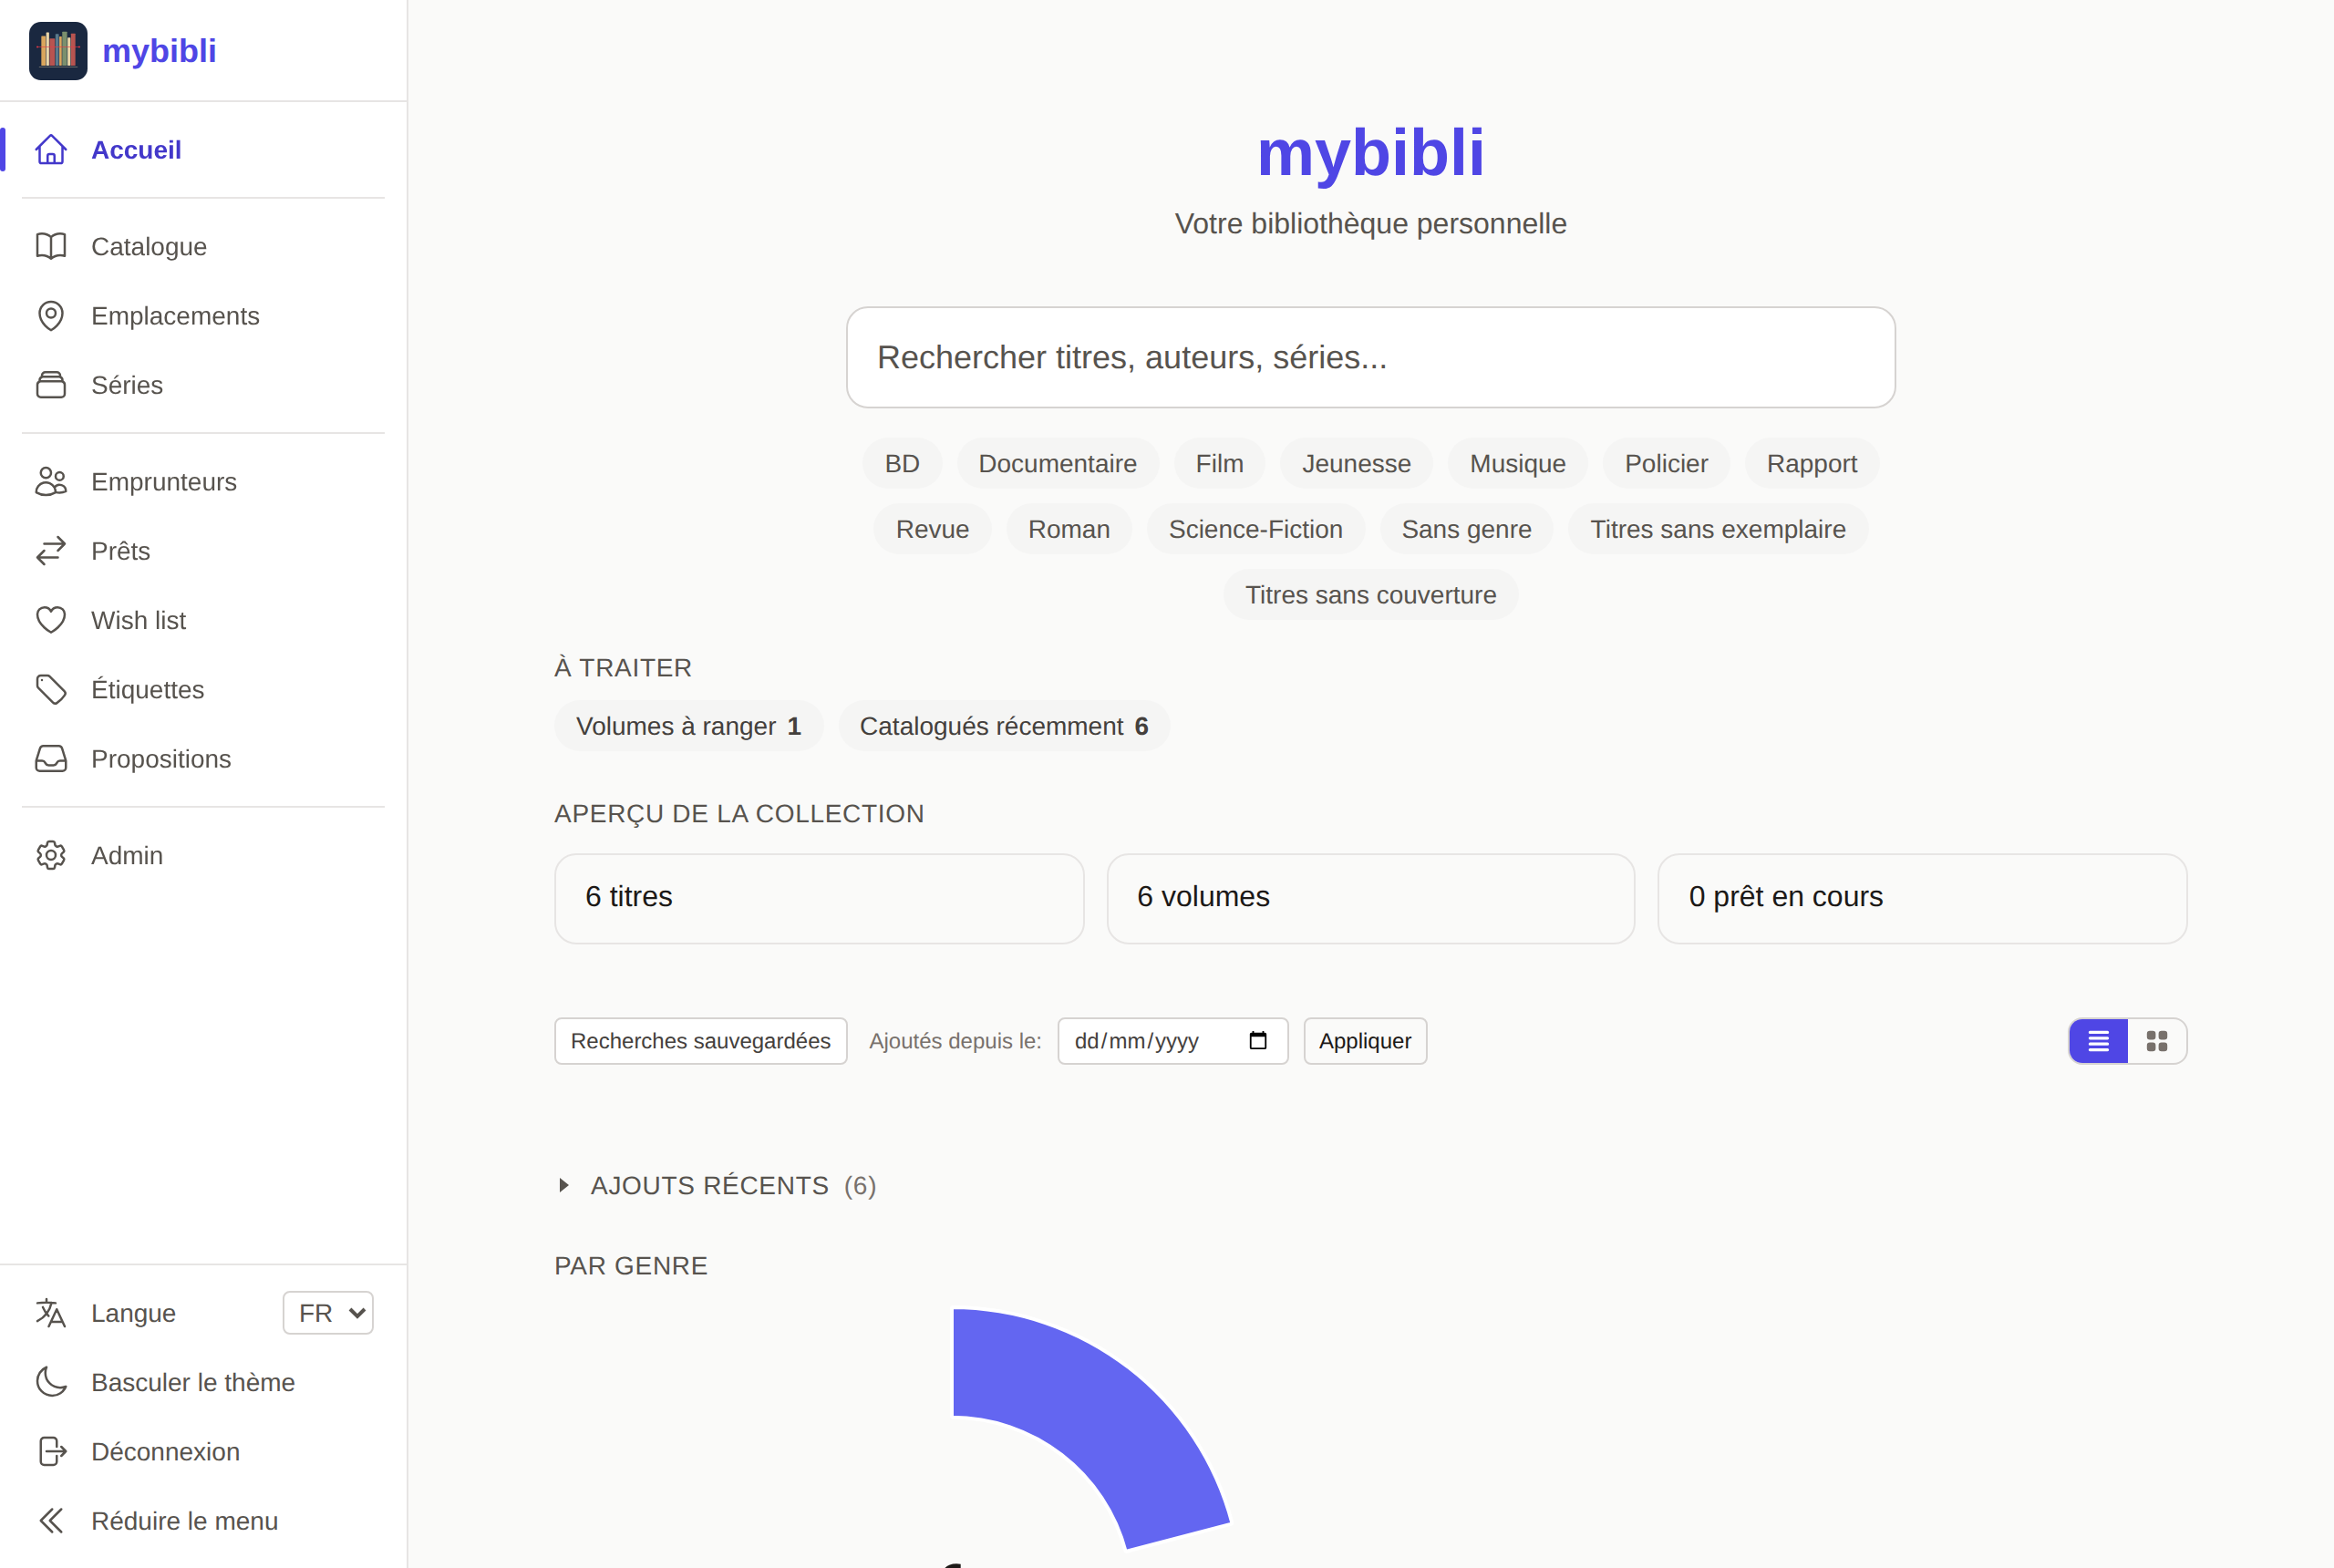
\includegraphics[width=0.95\textwidth]{01-home-desktop-fr.png}
  \caption{La page d'accueil dans une fenêtre de 1280\,px, connecté
    en Admin~: à gauche la barre latérale déployée (langue, thème et
    Déconnexion à son pied, le bouton pour la réduire en dessous),
    puis le champ de recherche, les puces de filtres par genre, les
    compteurs «~À traiter~» et les totaux «~Aperçu de la
    collection~».}
  \label{fig:home}
\end{figure}

La page d'accueil est le tableau de bord. De haut en bas :

\begin{itemize}
  \item \textbf{Champ de scan.}\index{champ de scan} Un champ
        focalisé qui accepte un ISBN, un code V ou un code L. La
        couche scanner-guard route l'entrée vers la bonne page
        selon le préfixe. Un ISBN saisi à la main peut garder les
        tirets ou les espaces imprimés sur le livre
        (\texttt{978-2-205-00121-1}, \texttt{2 205 00121 3}) :
        mybibli les retire et traite l'ISBN-13 nu, au scan comme
        dans la recherche.
  \item \textbf{Bandeau d'indicateurs.} Ajouts récents, prêts en
        retard, séries avec lacunes, volumes non rangés — chaque
        clic ouvre la liste filtrée correspondante.
  \item \textbf{Activité récente.} Les sept derniers jours de
        catalogage et de retours. Un titre compte comme
        \emph{catalogué récemment} quand le titre lui-même, ou l'un de
        ses volumes, a été ajouté pendant ces sept jours
        (section~\ref{sec:added-since}).
  \item \textbf{Ajouts récents.} Les titres qui ont reçu quelque chose
        en dernier --- le titre lui-même ou un nouveau volume, selon ce
        qui est le plus récent. Ils suivent la bascule \emph{Vue liste}
        / \emph{Vue grille} du catalogue situé en dessous : en vue
        liste, ils apparaissent dans le même tableau (avec sa colonne
        \emph{Ajouté}), en vue grille sous forme de cartes. La bascule
        change les deux à la fois, et le choix est conservé à la visite
        suivante.
\end{itemize}

\section{Cataloguer un nouveau titre via code-barres}\label{sec:catalog-scan}

\begin{enumerate}
  \item Focalisez le champ de scan de la page d'accueil (il est
        sélectionné par défaut au chargement). Scannez l'ISBN /
        EAN-13 du dos de l'ouvrage.
  \item mybibli redirige vers la page de catalogage, qui affiche un
        titre squelette avec le code-barres scanné. Une tâche
        d'arrière-plan lance des requêtes contre la chaîne de
        fournisseurs de métadonnées.
  \item En quelques secondes, le squelette se remplit : titre,
        contributeurs, éditeur, année, image de couverture. Un
        petit indicateur confirme quel fournisseur a résolu le
        titre.
  \item Choisissez un \textbf{lieu}\index{lieu} dans le menu
        déroulant (ou scannez le code L du rayon de destination) et
        un \textbf{état de volume}\index{état de volume}
        (typiquement \emph{Neuf}). Cliquez \textbf{Ajouter un
        volume}.
  \item Imprimez et collez une étiquette de code V sur le volume.
\end{enumerate}

Si le pipeline de métadonnées échoue à résoudre l'ISBN, le titre
apparaît avec un badge \emph{Non résolu}. Vous pouvez modifier les
champs manuellement et le volume est créé malgré tout.

\begin{tip}
Le catalogage en série marche le mieux quand la planche de codes V,
la douchette et l'imprimante sont à portée de main. La plupart du
temps est consacré à scanner, pas à attendre mybibli — la
récupération de métadonnées est asynchrone, vous n'avez donc pas à
attendre qu'elle se termine avant de passer au volume suivant.
\end{tip}

\subsection*{Scanner un code V déjà utilisé}
\label{sec:scan-existing-vcode}

Une pile de livres scannée en vitesse produit des répétitions. Depuis
la 1.23.0, mybibli les distingue au lieu de répondre à chacune par une
erreur :

\begin{itemize}
  \item \textbf{Une double lecture de la douchette.} Le même code
        arrivant deux fois en moins d'une seconde dans le même champ de
        scan n'est lu qu'une fois : la seconde lecture est ignorée sans
        message et le champ est vidé. Cela vaut pour tous les types de
        code. Le même code scanné à nouveau après cette seconde est
        traité normalement.
  \item \textbf{Un code V du titre en cours.} Scanner à nouveau l'ISBN
        et le code V d'un livre déjà catalogué (sans lieu actif) ne
        crée rien ; un message d'information l'indique : \emph{« Le
        label V0042 est déjà enregistré pour ce titre. »}
  \item \textbf{Un code V d'un autre titre.} Le code V n'est pas
        déplacé et rien n'est créé. Un avertissement nomme le titre qui
        le porte, avec son ISBN s'il en a un, renvoie à la page du
        volume, et suggère de scanner un autre label pour le livre
        en main ou d'ouvrir le volume : depuis sa page, on peut le
        déplacer vers le bon titre (section~\ref{sec:move-volume-title}).
  \item \textbf{Un rangement qui n'a pas eu lieu.} Avec un lieu actif,
        scanner un code V range le volume à cet endroit. Si la
        modification n'a pas pu être enregistrée, ou si le lieu actif a
        été supprimé entre-temps, le message dit que le volume
        \emph{n'a pas été rangé} et ce qu'il faut faire (scanner à
        nouveau le code V, ou scanner un autre code L) ; un lieu actif
        supprimé est abandonné.
\end{itemize}

\subsection*{Imprimer de nouvelles planches d'étiquettes}

Avant d'imprimer une nouvelle planche d'étiquettes V ou L, consultez
la petite ligne en haut de la page de catalogage (depuis la 1.12.0,
Librarian et plus) : \emph{« Étiquettes utilisées jusqu'à
V0142~·~L0037 — imprimez les nouvelles planches à partir des numéros
suivants. »} Les numéros incluent les éléments actuellement à la
corbeille — une étiquette imprimée et collée un jour sur un livre ne
sera jamais reproposée, même si ce volume a été supprimé depuis.

\section{Rechercher dans la collection}\label{sec:search}

La page \texttt{/search} accepte :

\begin{itemize}
  \item \textbf{titre} complet ou partiel ;
  \item \textbf{nom de contributeur} (matche l'auteur par défaut ;
        les autres rôles de contributeur sont scorés moins fort) ;
  \item \textbf{ISBN / EAN-13} — match exact ;
  \item \textbf{code V} ou \textbf{code L} — match exact ;
  \item \textbf{code Dewey} (pour les bibliothèques qui utilisent
        Dewey).
\end{itemize}

Les résultats sont triés par pertinence. Cliquez un résultat pour
ouvrir la page du titre ; cliquez un contributeur pour filtrer le
catalogue sur ses œuvres ; cliquez le libellé d'un lieu pour voir
chaque volume actuellement à cet endroit.

\begin{tip}
Vous pouvez « rechercher » un seul volume en scannant son code V
depuis n'importe quelle page qui dispose du champ de scan d'accueil
— y compris la page d'accueil, \texttt{/search} et \texttt{/loans}.
Plus rapide que la frappe.
\end{tip}

\subsection{Recherches sauvegardées}\label{sec:saved-searches}

Les recherches récurrentes (« BD sans couverture », « titres non
classés », « tout ce qui est en retard ») peuvent être sauvegardées
une fois puis relancées d'un seul clic. Sur la page d'accueil,
composez la recherche voulue — saisissez une requête, cliquez une
puce de filtre, choisissez un tri — puis ouvrez le menu déroulant
\textbf{Recherches sauvegardées} à côté du contrôle de tri et utilisez
\emph{Sauver la recherche courante} pour la nommer et l'enregistrer.

Les recherches sauvegardées sont \textbf{partagées par toute
l'instance} : tous les bibliothécaires voient et peuvent lancer le
même ensemble. Pour en lancer une, ouvrez le menu et cliquez son nom
— la page d'accueil se recharge avec cette requête, ce filtre et ce
tri appliqués. Chaque entrée propose aussi \emph{Renommer} et
\emph{Supprimer} (confirmation par fenêtre modale). La suppression est
réversible : sauvegarder une nouvelle recherche du même nom restaure
l'ancienne.

\begin{note}
Les recherches sauvegardées capturent les critères de navigation
existants (requête, une puce de filtre, colonne et sens de tri) — ce
n'est pas un constructeur de requêtes libre. Le contrôle n'est visible
que pour les bibliothécaires et les administrateurs. La date « ajoutés
depuis le » décrite ci-dessous n'est pas enregistrée avec une
recherche ; le formulaire d'enregistrement le signale tant qu'un filtre
de date est actif.
\end{note}

\subsection{Ce qui a été ajouté depuis un jour donné}\label{sec:added-since}

Depuis la 1.23.0, chaque page de titre et chaque page de volume
affichent, sous leurs champs principaux, \emph{Ajouté le} (le jour où
la fiche a été saisie) et \emph{Modifié le} (sa dernière modification,
téléchargements automatiques de métadonnées compris), dans le format
de date de la langue de l'interface.

Un titre compte comme \emph{ajouté} pendant une période quand le titre
lui-même y a été saisi \emph{ou} que l'un de ses volumes l'a été : un
titre ancien qui a reçu un nouvel exemplaire la semaine dernière fait
partie des ajouts de la semaine dernière. La même règle vaut à trois
endroits :

\begin{itemize}
  \item le champ de date \textbf{Ajoutés depuis le}, à côté du contrôle
        de tri du catalogue de la page d'accueil : choisissez un jour
        puis \emph{Appliquer} ; seuls restent les titres ajoutés depuis
        ce jour (\emph{Effacer} retire le filtre). La date figure dans
        l'adresse (\texttt{added\_since=AAAA-MM-JJ}) et se combine avec
        le texte recherché et le tri ;
  \item la colonne \textbf{Ajouté} du tableau du catalogue et les
        entrées correspondantes du menu de tri : la date d'un titre y
        est celle de son dernier ajout (la plus récente entre la sienne
        et celle de son volume le plus récent), les plus récents
        d'abord au premier clic ;
  \item l'indicateur \emph{Catalogués récemment} du tableau de bord,
        sur ses sept jours.
\end{itemize}

\begin{note}
Trois précisions. Les jours sont découpés à minuit UTC, pas à minuit
heure locale : en Suisse, un volume saisi entre minuit et 1~h (2~h en
été) compte pour la veille, et les dates affichées sur les pages sont
elles aussi des jours UTC. Un filtre d'indicateur (\emph{Catalogués
récemment}, \emph{Prêts en retard}, \dots) remplace le filtre de date, comme
il remplace le texte recherché --- un seul filtre actif à la fois.
Enfin, une recherche sur un ISBN ou un code V exact trouve son titre
quelle que soit la date, comme elle ignore déjà le filtre de genre.
\end{note}

\section{Étiquettes de gestion}\label{sec:management-labels}

Un genre dit ce qu'un livre \emph{est}. Un état dit comment un
exemplaire a \emph{vieilli}. Ni l'un ni l'autre ne dit « je ne suis pas
sûr que cette notice soit juste, il faudra y revenir » --- et c'est la
phrase dont un catalogue vivant a le plus besoin. Depuis la 1.18.0, les
\emph{étiquettes de gestion}\index{étiquette!de gestion} la portent.

Ce ne sont pas les étiquettes de dos de la section~\ref{sec:labels} :
rien ne s'imprime, rien ne se scanne, et un visiteur anonyme ne les voit
jamais. Elles existent pour la personne qui tient la bibliothèque.

\subsection*{Définir le vocabulaire}

Un administrateur crée le vocabulaire une fois, dans
\emph{Administration \textrightarrow{} Données de référence
\textrightarrow{} Étiquettes} : « À vérifier », « À relire », « Reliure
abîmée », « Prêté sans fiche » --- ce que votre pratique réclame. On les
renomme et on les supprime au même endroit, et comme toute autre valeur
de référence elles ne sont jamais traduites : ce que vous saisissez est
ce que tout le monde voit, quelle que soit la langue de l'interface.

Gardez la liste courte. Un vocabulaire de six étiquettes s'utilise ;
un vocabulaire de trente est une seconde taxonomie de genres que
personne n'entretient.

\subsection*{Poser une étiquette}

Un bibliothécaire pose les étiquettes depuis la section
\emph{Étiquettes} d'une page de titre ou d'une page de volume, en
choisissant dans ce vocabulaire commun. La distinction compte :

\begin{itemize}
  \item sur un \textbf{titre}, l'étiquette parle de la notice --- « les
        métadonnées ont l'air fausses » ;
  \item sur un \textbf{volume}, elle parle de cet exemplaire physique
        --- « celui-ci a la reliure abîmée », ce qui ne dit rien des
        deux autres exemplaires du rayon.
\end{itemize}

\subsection*{Retrouver ce qui porte une étiquette}

\texttt{/labels} liste le vocabulaire avec un compte en regard de chaque
entrée. En ouvrir une montre ce qui la porte, en deux sections --- les
titres au-dessus des volumes --- chaque ligne menant à sa page de
détail. C'est tout l'intérêt : une étiquette d'où l'on ne peut pas
revenir est un mot dans un tiroir.

\subsection*{Marquer les notices douteuses}

Une étiquette de gestion sert aussi à mettre de côté une notice dont
on doute : un ISBN qui semble appartenir à un autre livre, un volume
catalogué sous le mauvais titre, une description dans la mauvaise
langue. Créez une fois une étiquette pour cela --- par exemple
\emph{Code douteux} ---, posez-la sur le titre ou le volume concerné, et
sa page \texttt{/labels/\{id\}} devient la liste des notices à
reprendre. Une fois la notice corrigée, retirez-lui l'étiquette. Il n'y
a pas de liste d'« anomalies » à part ni de champ de motif : le nom de
l'étiquette dit de quel doute il s'agit.

Un agent IA qui travaille sur le catalogue peut \emph{proposer} une
telle étiquette sur un titre ou un volume ; la proposition apparaît
sur la page Propositions et l'étiquette n'est posée que si vous
l'acceptez (section~\ref{sec:agents-tools}).

\begin{note}
Les étiquettes sont internes. Les gestionnaires n'exécutent même pas les
requêtes pour un visiteur anonyme : rien ne fuit par le catalogue
public --- pas même le fait qu'une étiquette existe.
\end{note}

\section{Déplacer un volume vers un autre lieu}\label{sec:move-volume}

\begin{enumerate}
  \item Ouvrez la page du volume (recherche par code V ou clic
        depuis la page du titre).
  \item Cliquez \textbf{Déplacer}.
  \item Scannez le code L du lieu de destination, ou choisissez-le
        dans le menu déroulant.
  \item Confirmez.
\end{enumerate}

mybibli enregistre le déplacement dans l'historique de lieu du
volume, vous permettant de retracer où un livre a vécu au fil du
temps.

Partout où une liste de volumes indique leur lieu --- le tableau et les
cartes des volumes d'une page de titre, la page d'une étiquette de
gestion, la liste d'audit ---, ce lieu est donné par son chemin
complet, par exemple \emph{Maison \textrightarrow{} Salon
\textrightarrow{} Bibliothèque \textrightarrow{} Étagère 3 (L0042)} :
deux étagères « Étagère 3 » dans deux pièces différentes ne se
confondent plus. Un chemin long passe à la ligne sur un écran étroit.
La page d'un lieu ne liste que les volumes rangés directement à cet
endroit, sous son propre chemin complet.

\section{Rattacher un volume à un autre titre}\label{sec:move-volume-title}

Un code V collé sur le mauvais livre, ou scanné alors que le mauvais
titre était en cours --- typiquement un EAN d'éditeur partagé par
plusieurs albums ---, laisse un volume sous un titre qui n'est pas le
sien. Depuis la 1.23.0, on peut le déplacer sans le supprimer :

\begin{enumerate}
  \item Ouvrez la page du volume (Bibliothécaire ou Admin) et cliquez
        \textbf{Déplacer vers un autre titre}.
  \item Dans la fenêtre, cherchez le bon titre par son titre ou son
        ISBN (tirets et espaces admis). Dix titres au plus sont
        proposés ; le titre actuel du volume ne l'est jamais.
  \item Choisissez-en un. Une phrase nomme le volume, son titre actuel
        et le titre cible, et rappelle que son label, son emplacement
        et ses prêts le suivent.
  \item Cliquez \textbf{Déplacer}.
\end{enumerate}

La page du volume affiche alors le nouveau titre, et les deux pages de
titre listent le volume là où il se trouve désormais. Tout ce qui
appartient au volume le suit : son code V, son lieu, son état, ses
valeurs, ses étiquettes de gestion, son drapeau d'audit et ses prêts
--- y compris un prêt en cours, qui le suit simplement. Les positions
dans les séries et les tomes attendus appartiennent aux titres et ne
sont pas touchés. Le déplacement est consigné dans le journal
(\emph{Volume moved to another title}, avec le volume, les deux titres
et l'utilisateur).

Le déplacement est refusé, avec une explication dans la fenêtre,
quand aucun titre n'a été choisi, quand la cible est le titre actuel du
volume, quand la cible ou le volume a été supprimé entre-temps, ou quand
quelqu'un d'autre a modifié le volume depuis l'ouverture de la fenêtre
(rechargez la page et recommencez).

\section{Séries et numéros de tome}\label{sec:tome-number}

Un titre se place dans une série depuis la section \emph{Séries} de sa
page : choisissez la série, indiquez la position, attribuez. Le menu
propose toutes les séries de la bibliothèque, par ordre alphabétique.

\subsection*{Le numéro de tome}

La position d'un titre dans sa série \emph{est} son numéro de tome.
Depuis la 1.23.0, elle s'affiche comme tel : sous le titre de la page
(\emph{« Tome 3 · Thorgal »} ; \emph{« Volume 3 · Thorgal »} dans
l'interface anglaise), sur les lignes et les cartes du catalogue, sur
la page de la série et sur la page du volume. Une intégrale affiche
\emph{« Tomes 3--5 »} ; un titre présent dans plusieurs séries affiche
une mention par série.

Pour le changer, cliquez \textbf{Modifier} à côté de la série, dans la
section \emph{Séries} de la page du titre, saisissez la nouvelle
position puis \textbf{Enregistrer}. Les règles sont celles d'une
attribution : une position d'au moins 1, dans les limites du nombre de
volumes d'une série fermée, et pas une position que le titre occupe
déjà dans cette série (deux titres différents peuvent partager une
position : la page de la série le montre, elle ne l'empêche pas). La
plage d'une intégrale ne se modifie pas là : retirez-la de la série
puis attribuez-la à nouveau. Après la modification, les tomes attendus
sont réévalués --- la position quittée redevient une lacune, la
nouvelle peut résoudre un tome attendu (section~\ref{sec:expected-tomes}).

\subsection*{Les mentions de tome dans les titres téléchargés}

Les fournisseurs mettent souvent le numéro dans le titre : \emph{«
Thorgal - Tome 29 - Le sacrifice »}, \emph{« Titeuf T12 : \dots »}.
Quand un téléchargement de métadonnées fixe un titre (au scan, par
\emph{Re-télécharger les métadonnées}, lors d'une nouvelle tentative
automatique ou d'un traitement en lot), mybibli retire cette
mention\index{mention de tome} --- \emph{« Thorgal - Le sacrifice »}
---, pourvu que le titre n'ait jamais été modifié à la main. Ce qui
compte comme mention dépend du type de média :

\begin{itemize}
  \item \textbf{Bandes dessinées} : \emph{Tome}, \emph{Tomo}, \emph{T},
        \emph{T.}, \emph{Vol.}, \emph{Volume}, \emph{Band}, \emph{Bd.},
        \emph{n°}, \emph{No}, \emph{\#}, suivis d'un nombre ;
  \item \textbf{Livres} : seulement \emph{Tome}, \emph{Tomo},
        \emph{Volume}, \emph{Vol.} et \emph{Band}, et un nombre de 1000
        ou plus est pris pour une année, pas pour un tome ;
  \item autres types de média : jamais.
\end{itemize}

La mention doit se trouver au début du titre, à sa fin, ou entre deux
parties séparées par un deux-points, un tiret, une virgule ou un point.
Un titre qui porte plusieurs mentions, une plage ou une liste
(\emph{« Intégrale T1 à T3 »}, \emph{« T1 - 3 »}) est laissé tel quel.
Pour une bande dessinée dont le titre ne porte aucune mention, c'est le
numéro dans la collection de la notice de bibliothèque nationale qui
est retenu.

Le numéro retiré du titre ne devient une position dans une série que
si vous la fixez :

\begin{itemize}
  \item un titre \textbf{hors de toute série} le garde comme indice,
        affiché sous le titre de la page : \emph{« Tome 3 (détecté)~»}. Quand vous attribuez ensuite une série depuis la page du
        titre, le champ de position en est déjà rempli. L'indice
        disparaît dès que le titre est dans une série ; il ne fait
        jamais foi ;
  \item un titre \textbf{déjà dans une série} garde ses positions
        telles quelles.
\end{itemize}

Avec \emph{Re-télécharger les métadonnées}, l'aperçu montre le titre
déjà nettoyé ; l'indice est enregistré quand vous confirmez ce titre.

Un titre que vous saisissez vous-même --- à la création ou dans le
formulaire de modification --- n'est jamais réécrit. S'il contient une
mention, un message suggère de retirer le numéro du titre et de
l'indiquer comme position dans la série.

\begin{warning}
La reconnaissance est volontairement prudente, mais quelques titres de
bande dessinée ont la forme d'une mention dans leur nom même :
\emph{« L'Ennemi public n°1 »}, \emph{« Le Prisonnier n°6 »},
\emph{« Public Enemy \#1 »}, \emph{« Panzer T34 : \dots »}. Ils perdent
leur numéro au téléchargement. Corrigez le titre une fois à la main :
un titre modifié à la main est protégé, et aucun téléchargement
ultérieur ne le change plus.
\end{warning}

Les titres catalogués avant la 1.23.0 gardent leurs mentions : il n'y a
pas de nettoyage en lot. Un agent IA peut proposer les corrections ---
le titre par une proposition de métadonnées, la position par une
proposition de série (chapitre~\ref{ch:agents}).

\section{Prêts}\label{sec:loans}

\subsection*{Prêter un volume}

\begin{enumerate}
  \item Ouvrez \texttt{/loans} et cliquez \textbf{Nouveau prêt}.
  \item Scannez ou choisissez l'\textbf{emprunteur}\index{emprunteur}.
        Si l'emprunteur n'existe pas encore, cliquez \emph{Créer
        l'emprunteur} en ligne.
  \item Scannez ou choisissez le \textbf{volume} (code V).
  \item Réglez optionnellement une \textbf{date de retour
        prévue} ; sinon mybibli la calcule à partir du seuil de
        retard (chapitre~\ref{ch:configuration}).
  \item Confirmez.
\end{enumerate}

Le lieu actuel du volume est inscrit sur la ligne de prêt pour
qu'un retour ultérieur puisse le restaurer au bon rayon.

\subsection*{Retourner un volume}

\begin{enumerate}
  \item Ouvrez \texttt{/loans} et trouvez le prêt actif (filtre
        \emph{Actifs} ou scan du code V).
  \item Cliquez \textbf{Retourner}.
  \item Choisissez l'état post-retour (\emph{Bon}, \emph{Usé},
        \dots).
  \item Confirmez. Le volume retourne automatiquement à son lieu
        d'avant prêt.
\end{enumerate}

\subsection*{Prêts en retard}

Les prêts qui dépassent le seuil de retard passent au rouge sur la
page \texttt{/loans} et sur l'indicateur \emph{En retard} de la page
d'accueil. \texttt{/loans?filter=overdue} donne une liste focalisée.

\section{Audit des rayons}\label{sec:audit}

Un \emph{audit}\index{audit} c'est le rituel « je parcours les
étagères et je confirme que tout est bien à la place que la base
indique ». Depuis la 1.7.x, mybibli porte ce flux au lieu de vous
laisser l'improviser autour de la page de recherche.

L'unité de travail est un drapeau posé sur un volume :
\emph{à contrôler}. On lève le drapeau, on parcourt le rayon, et on
l'abaisse à mesure que chaque exemplaire est confirmé.

\subsection*{Lever le drapeau}

\begin{itemize}
  \item \textbf{Un volume} — depuis sa page de détail,
        \emph{Marquer à contrôler}. Utile quand un lecteur signale que
        quelque chose cloche, ou qu'un scan a fait apparaître un volume
        là où il n'aurait pas dû être.
  \item \textbf{Un rayon entier} — depuis la page d'un lieu de
        rangement, \emph{Marquer tous les volumes à contrôler}. C'est
        ainsi qu'une passe planifiée commence : on marque le rayon le
        dimanche soir, on le parcourt dans la semaine.
\end{itemize}

Un volume marqué porte une pastille \emph{À contrôler} partout où il
est listé : le drapeau se voit sans ouvrir la vue d'audit.

\subsection*{Parcourir le rayon}

Le tableau de bord d'accueil affiche un indicateur \emph{Volumes à
contrôler} avec son compte et un lien ; \texttt{/audit} est la liste
elle-même, triée par lieu puis par code V — l'ordre dans lequel on
marche. Chaque ligne porte un bouton \emph{Contrôlé} : on l'actionne
quand on tient l'exemplaire, et la ligne quitte la liste.

Deux situations se dénouent en chemin :

\begin{itemize}
  \item Un volume sur le rayon que la liste n'attend pas — scannez-le ;
        mybibli signale qu'il appartient ailleurs et vous le déplacez
        (section~\ref{sec:move-volume}).
  \item Un volume que la liste attend et que le rayon ne porte pas —
        laissez le drapeau levé. Une liste d'audit inachevée est une
        liste de choses à faire, pas un échec : c'est le seul relevé de
        ce que vous n'avez pas retrouvé.
\end{itemize}

\emph{Effacer tous les drapeaux} vide la liste d'un coup. À utiliser
quand on abandonne une passe, pas pour en terminer une — un drapeau
effacé sans avoir le volume en main enregistre une vérification qui
n'a pas eu lieu.

\begin{tip}
Un audit trimestriel attrape les volumes mal rangés tôt — plus un
livre traîne au mauvais rayon, plus il est difficile de se rappeler
où il aurait dû être.
\end{tip}

\section{Rangement après retours}\label{sec:shelving}

Après une fournée de retours, les volumes s'empilent près du poste
de scan. Le flux de \emph{rangement}\index{rangement} de mybibli
accélère la remise en rayon :

\begin{enumerate}
  \item Prenez un volume et scannez son code V.
  \item mybibli affiche la page du volume avec le lieu d'origine
        bien en évidence.
  \item Portez le volume au rayon indiqué. Scannez le code L du
        rayon pour confirmer.
  \item Recommencez.
\end{enumerate}

La confirmation par code L est optionnelle mais recommandée — elle
laisse une entrée fraîche dans l'historique du volume sur laquelle
le prochain audit pourra s'appuyer.

\subsection{Annuler une action de scan}\label{sec:scan-undo}

Le travail au code-barres va vite, et une erreur de scan arrive
parfois — un volume rangé au mauvais lieu, ou un lieu de lot activé
par mégarde. Lorsque vous rangez un volume ou activez un lieu de lot
sur la page de catalogage, le message de confirmation affiche un
bouton \textbf{Annuler}. Cliquez-le dans les \textbf{30 secondes} et
mybibli annule cette dernière action :

\begin{itemize}
  \item Annuler un rangement remet le volume à son lieu précédent
        (ou le laisse non rangé s'il n'avait pas de lieu auparavant).
  \item Annuler l'activation d'un lieu de lot rétablit le lieu actif
        précédent.
\end{itemize}

Seule la \emph{dernière} action peut être annulée, et le bouton
disparaît une fois la fenêtre de 30 secondes écoulée. L'annulation ne
touche que le changement de lieu — elle ne supprime jamais un titre
ou un volume que vous venez de créer. Passé le délai, déplacez le
volume de la manière habituelle (\autoref{sec:move-volume}).

\section{Wish list}\label{sec:wishlist}

La \emph{wish list}\index{wish list} est une liste séparée des
livres que vous aimeriez acheter, distincte du catalogue possédé.
Elle vit sous \texttt{/wishlist}\index{wishlist@/wishlist} (entrée
\textbf{Wish list} de la barre latérale) et est disponible pour les Bibliothécaires
et les Admins. Un tome manquant d'une série s'y ajoute d'un clic
depuis la page de la série (section~\ref{sec:expected-tomes}).

\subsection{Ajouter une entrée}

Le formulaire \emph{Ajouter à la wish list} propose deux modes~:

\begin{itemize}
  \item \textbf{Par ISBN.} Scannez ou saisissez un ISBN à 13
        chiffres. mybibli interroge la même chaîne de fournisseurs
        de métadonnées que le catalogue, puis affiche une carte de
        prévisualisation (titre, auteur, éditeur, année,
        couverture). Cliquez sur \emph{Ajouter à la wish list}
        pour enregistrer. Les images de couverture pointent
        directement sur l'URL du fournisseur résolu (Open Library
        Covers ou Google Books par exemple)~; le téléchargement
        local de la couverture est sur la roadmap.
  \item \textbf{Saisie libre.} À utiliser quand vous n'avez pas
        d'ISBN sous la main (titre auto-édité, recommandation
        notée pendant le déjeuner). Seul le \emph{Titre} est
        obligatoire~; auteur, éditeur et notes sont optionnels.
\end{itemize}

\subsection{Parcourir en librairie}

La vue liste se transforme en pile de cartes sur les petits
écrans \string— conçue pour parcourir rapidement d'un pouce dans
une librairie. Chaque carte affiche le titre, l'auteur (s'il est
connu), l'ISBN (s'il y en a un), l'éditeur et la date d'ajout.

Pour imprimer une copie papier ou sauver un PDF pour usage
hors-ligne, cliquez sur \emph{Imprimer} en haut de la liste.
mybibli rend une page d'impression épurée~; utilisez \emph{Imprimer
en PDF} du navigateur (Fichier \string→ Imprimer \string→
Enregistrer en PDF, ou Ctrl/Cmd-P) pour générer un PDF à
emporter à la librairie.

\subsection{Marquer un livre comme acheté}

Quand vous achetez un livre, ouvrez son entrée wish list (ou
tapez \emph{Acheté} directement depuis la ligne de la liste),
confirmez dans la modale, et l'entrée est mise en
soft-delete. L'action est réversible depuis le panneau Corbeille
de l'admin pendant 30 jours.

\subsection{Auto-détection au scan catalogue}

Quand vous cataloguez un livre fraîchement acheté via le flux
standard de scan (\texttt{/catalog}), mybibli vérifie si son ISBN
correspond à une entrée wish list active. Si oui, un bandeau
émeraude apparaît dans la zone de feedback~: \emph{Cet ISBN est
sur votre wish list \string— la retirer~?} Un clic sur le bouton
\emph{Retirer de la wish list} ouvre la même modale \emph{Marquer
comme acheté}, et la confirmation supprime l'entrée. Aucune
suppression silencieuse.

\section{Ce que vaut la bibliothèque}\label{sec:valuation}

Deux montants facultatifs peuvent être enregistrés sur chaque volume :
ce qu'il vous a \emph{coûté} (prix d'achat) et ce qu'il \emph{vaut}
aujourd'hui (valeur actuelle), chacun avec sa devise. Les deux sont
vides par défaut et rien ne force à les remplir --- une bibliothèque qui
n'est pas un placement peut ignorer cette section.

Si vous les renseignez, \texttt{/stats/value}\index{valorisation} en
fait la somme sur tout le catalogue : un total par devise, puis une
ventilation par genre et par série. Les volumes sans valeur sont
ignorés plutôt que comptés à zéro : un catalogue partiellement valorisé
dit donc la vérité sur la partie que vous avez valorisée, au lieu de
diluer la moyenne.

\begin{itemize}
  \item La \textbf{devise par défaut} des nouvelles valorisations se
        règle dans \emph{Administration \textrightarrow{} System} ; ce
        n'est qu'un pré-remplissage, chaque volume peut en porter une
        autre.
  \item La \textbf{carte du tableau de bord} qui affiche le total estimé
        est \emph{désactivée} par défaut. Activez-la au même endroit si
        vous voulez ce chiffre sous les yeux chaque jour --- ce n'est pas
        le souhait de tous les foyers.
\end{itemize}

\subsection*{Couverture}

Depuis la version 1.25.0, la page s'ouvre sur la \textbf{couverture} de
ces totaux : combien de volumes la bibliothèque compte, combien portent
une valeur actuelle et quelle part cela représente, les dates de
l'estimation la plus ancienne et de la plus récente, et combien
d'estimations ont plus d'un an --- ou n'ont pas de date --- et méritent
d'être revues. Les mêmes chiffres sont donnés par genre et par série,
les moins couverts d'abord. Un total qui repose sur le dixième de la
collection, ou sur des estimations vieilles de plusieurs années, le dit.
Un agent IA peut aider (chapitre~\ref{ch:agents}) : il liste d'abord
les volumes jamais estimés et propose des valeurs que vous acceptez ou
refusez (section~\ref{sec:proposals-series-value}). Les totaux laissent
de côté les volumes des titres supprimés.

\begin{note}
L'assurance est la raison habituelle de tenir ces chiffres. Si c'est la
vôtre, notez le prix d'achat autant que la valeur actuelle : le premier
est un fait que vous pouvez prouver, la seconde une estimation qu'on
vous demandera de justifier.
\end{note}
